\chapter{Conclusion}
\label{ch:conclusion}

In this chapter we provide our final set of metrics for the performance of the original isogeny-based signature scheme, our batched inversion implementation of the protocol, and our implementation feauturing $\psi(S)$ compression. We also offer measurements for how the compressed version of the protocol performs when combined with batched inversion. We outline also how the compressed protocol offers an additional route for batching inversions, yielding further performance improvements.

Following the debriefing of our results, we offer one final section wherein we discuss the ramifications of our work in a general context. In this section we also discuss some possible future work to further progress the practicality of isogeny-based cryptography.



\section{Performance Results}

In this section we compile performance metrics for the original Yoo et al. signature scheme, our batched-inversion signature scheme, our compressed signature scheme, and also our combined compression with batched inversions implementation. For each of these implementations we show the average cycle time for \textbf{Sign} and \textbf{Verify} as well as the standard deviation. These measurements are outlined in \ref{fig:allmeasurements} (where ``C+B" denotes the combined compression with batching scheme).

\begin{figure}
\begin{center}
\begin{tabular}{ | l | b | b | }
\hline
& Average Cycles & Standard Deviation \\
\hline
Original Sign & 4,611,010,573.608 & 300,643,097.882 \\
Original Verify & 3,221,544,625.173 & 263,674,018.528 \\
Batched Sign & 4,552,062,482.520 & 18,113,276.904 \\
Batched Verify & 3,173,340,239.461 & 68,672,478.339 \\
Compressed Sign & a & b \\
Compressed Verify & a & b \\
C+B Sign & a & b \\
C+B Verify & a & b \\
\hline
\end{tabular}
\end{center}
\caption{Average performance and standard deviation in clock cycles for all versions of the Yoo et al. signature scheme.}
\label{fig:allmeasurements}
\end{figure}

We include graphical representations of our collected data, these can be found in \ref{fig:vanillacyclesgraph}, \ref{fig:batchedcyclesgraph}, \ref{fig:compressedcyclesgraph}, and \ref{fig:CBcyclesgraph}. The collected measurements for the unedited signature depicts several outliers taken at the beginning of data collection: this is quite likely attributed to time taken loading program data into RAM. The measurements that follow these outliers reflect the cycle time for the procedure once the code has been fetched and stored in memory. 

\begin{figure}
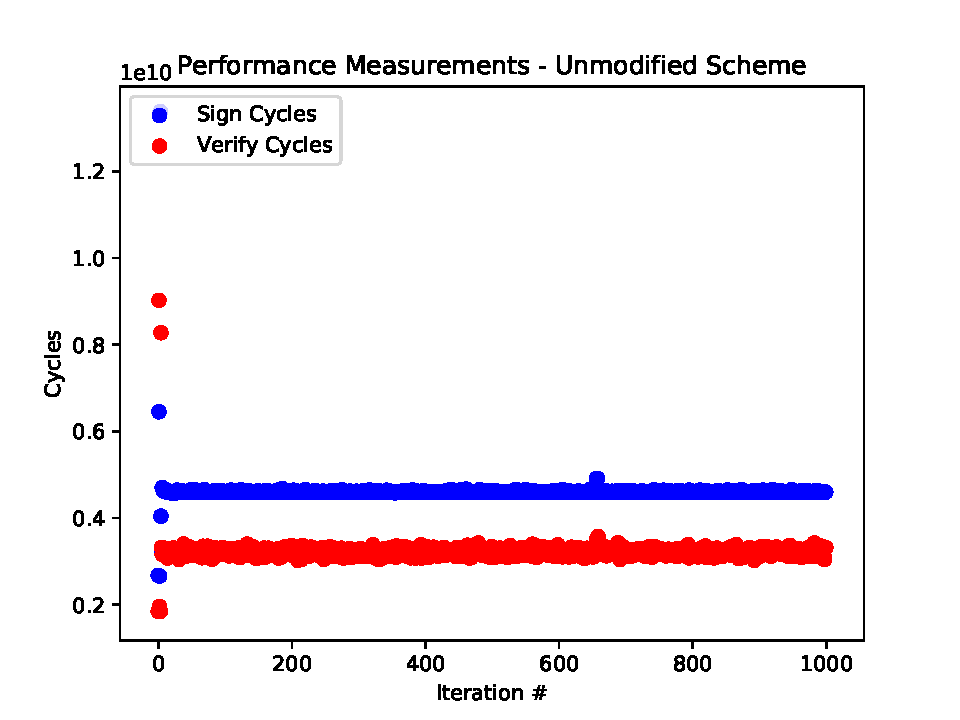
\includegraphics{vanilla-cycles.pdf}
\caption{Cycle times for 1,000 unedited Yoo et al. signatures.}
\label{fig:vanillacyclesgraph}
\end{figure}

\begin{figure}
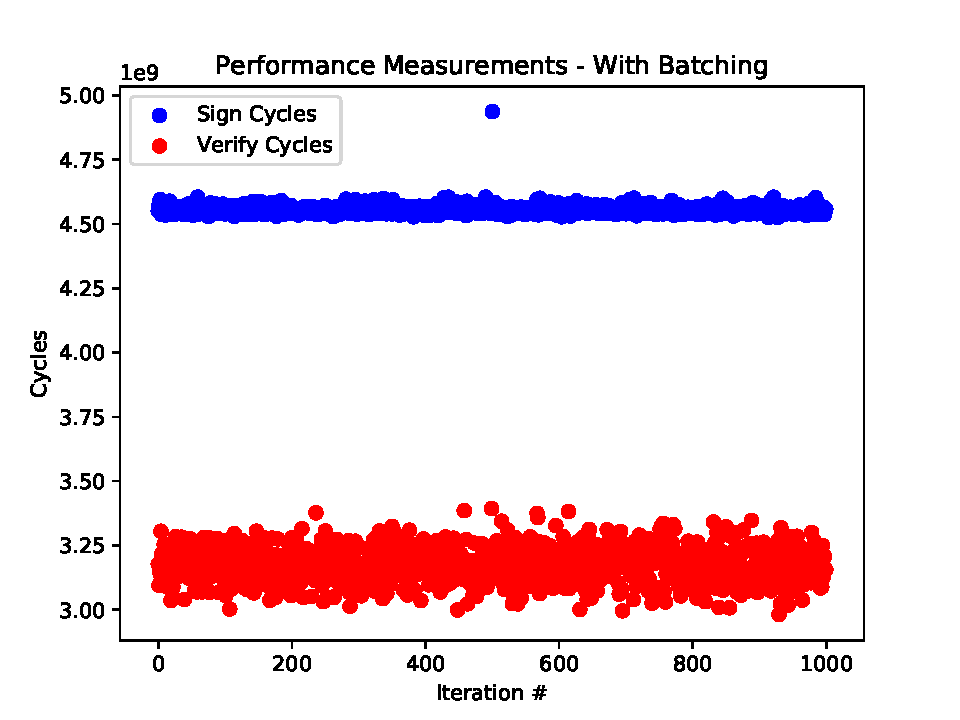
\includegraphics{batched-cycles.pdf}
\caption{Cycle times for 1,000 signature with batched inversions.}
\label{fig:batchedcyclesgraph}
\end{figure}

The reader might note that the the performance metrics of this protocol all yield a considerably high standard deviation. This can be attributed to a few factors. The first and perhaps most influential factor is the size of the private key value $m$. The larger $m$ is, the longer basic $\mathbb{F}_{p^2}$ arithmetic can take. This can be attributed to

We return again to the comparison charts employed in Section \ref{subsec:perfcomparisons} to compare the tomporal and spatial performance of these isogeny-based signatures to other post-quantum and classical alternatives. This time, we use the metrics resulting from our modified implementations as the point of comparison. These comparisons can be found in Figure \ref{fig:endperfcomparisons} (comparing subroutine performances) and Figure \ref{fig:endsizecomparisons} (compairing key and signature sizes). These metrics are all taken, yet again, at the 128-bit post quantum securty level (or classical security level, in the case of RSA and ECDSA).

\begin{figure}
\begin{center}
\begin{tabular}{ l | b | b | b }
\hline
\mc{1}{}  & \mc{1}{Key Gen} & \mc{1}{Sign} & \mc{1}{Verify}\\
\hline
\rowcolor{Gray}
SIDH & a & b & c \\
\rowcolor{light-green}
SIDH Batched & a & b & c \\
\rowcolor{light-green}
SIDH Compressed & a & b & c \\
\rowcolor{light-green}
SIDH C+B & a & b & c \\
Sphincs & a & b & c \\
Rainbow & a & b & c \\
qTESLA & a & b & c \\
Picnic & a & b & c \\
\rowcolor{light-red}
RSA & a & b & c \\
\rowcolor{light-red}
ECDSA & a & b & c \\
\hline
\end{tabular}
\end{center}
\caption{Performance in clock cycles for our improved isogeny-based signatures in comparison with other post-quantum and classical alternatives.}
\label{fig:endperfcomparisons}
\end{figure}

\begin{figure}
\begin{center}
\begin{tabular}{ l | b | b | b }
\hline
\mc{1}{}  & \mc{1}{Public Key} & \mc{1}{Private Key} & \mc{1}{Signature}\\
\hline
\rowcolor{Gray}
SIDH & 768 & b & 141,312 \\
\rowcolor{light-green}
SIDH Compressed & 768 & b & 141,312 \\
Sphincs & 32 & 64 & 8,080 - 16,976 \\
Rainbow & 152,097 - 192,241 & 100,209 - 114,308 & 64 - 104 \\
qTESLA & 4,128 & 2,112 & 3,104 \\
Picnic & 33 & 49 & 34,004 - 53,933 \\
\rowcolor{light-red}
RSA & 384 & b & 384 \\
\rowcolor{light-red}
ECDSA & 32 & b & 32 \\
\hline
\end{tabular}
\caption{Key and signature sizes for our compressed isogeny-based signatures in comparison with other post-quantum and classical alternatives.}
\label{fig:endsizecomparisons}
\end{center}
\end{figure}


\section{Discussion \& Concluding Remarks}

In this final section, we finish off the dissertation with some concluding remarks on the applicability of SIDH and isogeny-based cryptography, the importance of post-quantum cryptography, and the possible avenues for future work in this specific area. 

If one assumes security of the original SIDH key exchange protocol, then the Yoo et al. signature scheme is provably secure and requires no additional underlying assumptions. Given that \sidh keys are non-ephemeral, and so could pose a promising candidate in the context of TLS certificate signing. Certificate authority signatures, not requiring constant transfer over the wire (as they are offen packaged with Internet browsers or sperating systems) are less desperate for small signature sizes.

\subsection{Future Work}
\label{sec:morebatch}

The most direct line of future work that can

The next step for these implementations would be to merge them into the Microsoft SIDH public repository.

One additional scenario in which inversion batching can be utilized lies in server-client applications. Servers that are managing 
